% !TEX root = ./informe.tex
\section{Grasp}

\subsection{Explicación}
GRASP es sigla de Procedimientos Golosos Aleatorios Adaptativos de Búsqueda (Greedy Randomized Adaptive Search Procedures. Es una metaheurística que se basa en utilizar métodos golosos constructivos y de búsqueda local para resolver un problema computacionalmente dificil, utilizando el azar para no estancarse en un único máximo local. Cada iteración de un algoritmo GRASP construye golosamente una solución desde cero, admitiendo cierto grado de aleatoriedad al añadir elementos a la solución; para después mejorar el resultado con un método de búsqueda local. Realizamos varias iteraciones, deteníendonos bajo algún criterio de corte, ya sea por que conseguimos una solución lo suficientemente buena, o porque nos pasamos de una cantidad de iteraciones predeterminada. La mejor solución conseguida entre todas las iteraciones es el resultado final del algoritmo. \cite{paper_grasp} \\

El algoritmo goloso constructivo que va a ir un poco más allá del algoritmo \textit{golosoB} del que hablamos en la sección anterior. En vez de tomar el nodo inicial como parámetro y seguir con un algoritmo puramente greedy, en cada nuevo elemento admitiremos un poco de azar dentro de lo razonable. Para esto, en vez de maximizar de forma directa nuestra funcion greedy (cardinalidad de la frontera) sobre los nodos no agregados, construiremos una RCL (Restricted Candidate List). La misma contendrá los candidatos que cumplan con un cierto nivel de optimalidad, del que será elegido un nodo al azar para finalmente agregarse a la solución final. \\

El criterio con el cuál se tomarán candidatos al RCL estará dictaminado por un parámetro $alpha$, que indicará qué porcentaje del rango de valores posibles que pueden tomar los candidatos, se admiten en la RCL. Formalmente, un nodo $c$ que resulta en una frontera $f_c$ al ser agregado a la solución parcial, pertenece al RCL solo si $f_c \geq f_{max} + \alpha * (f_{min} - f_{max})$, con $max$ nodo localmente óptimo, y $min$ nodo localmente peor. A grandes rasgos, un $alpha$ grande implica darle más peso al azar, y uno más chico, a la porción golosa del algoritmo. (Notemos que para que esto tenga sentido, $\alpha \in \mathbb{R}$ y $0 \leq \alpha \leq 1$). Una vez que el RCL está formado, se elije un nodo al azar, y se comienza el proceso de nuevo, hasta no poder continuar. \\

Obtenida una solución inicial, como nuestro método no es (en general) completamente goloso, podemos utilizar un algoritmo de búsqueda local movernos hacia un máximo local, mejorando nuestra solución y completando una iteración de GRASP. El algoritmo que usamos para este propósito es el mismo de la sección anterior.

\subsection{Pseudocódigo}

Las funciones local.resolver(), EsClique() y Frontera() no son incluidas aquí por ser iguales a las incluidas previamente. Las complejidades son $O(n^5)$, $O(n^3)$ y $O(n^2)$ respectivamente.

Referencias de variables globales para el pseudocódigo:
\begin{itemize}
    \item $n$: La cantidad de nodos
    \item $solucion$: Secuencia que contiene la clique solución
\end{itemize}

\begin{algorithm}[H]
\begin{algorithmic}
\Function{Resolver}{$\alpha$, $repsGrasp$, $repsLocal$}
    \State $fronteraMax \gets 0$                    \Comment $O(1)$
    \State $fronteraNueva \gets 0$                  \Comment $O(1)$
    \State $reps \gets 0$                           \Comment $O(1)$
    \For{$reps \in$ [$1..repsGrasp$]}                           \Comment $O(repsGrasp * repsLocal * n^5)$
    % \While{$reps < repsGrasp$}  \Comment $What Goes Here$
        \State $actual \gets $GreedyRandom($\alpha$)              \Comment $O(n^5)$
        \State $nueva \gets$ local.resolver($actual, repsLocal$)  \Comment $O(repsLocal * n^5)$
        \State $fronteraNueva \gets$ Frontera($nueva$)            \Comment $O(n^2)$
        \If {$fronteraNueva > fronteraMax$}                     \Comment $O(1)$
            \State $solucion \gets nueva$                       \Comment $O(1)$
            \State $fronteraMax \gets fronteraNueva$            \Comment $O(1)$
        %     \State $reps \gets 0$   \Comment $O(1)$
        % \Else
        %     \State $reps \gets reps + 1$   \Comment $O(1)$
        \EndIf
    % \EndWhile
    \EndFor
    \State return $solucion$
\EndFunction
\end{algorithmic}
\end{algorithm}
Para calcular el $RCL$ hacemos un primer pasaje para calcular el máximo y el mínimo de los nodos candidatos a agregarse al clique parcial. En una segunda pasada es cuando vamos agregando los nodos a medida que encontramos aquellos que cumplen con la fórmula planteada en la Explicación.

\begin{algorithm}[H]
\begin{algorithmic}
\Function{GreedyRandom}{$\alpha$}
    \State $fronteraMax \gets -1$                       \Comment $O(1)$

    \State $candidatosInicial \gets \{1..n\}$         \Comment $O(n)$

    \State $solucion \gets \emptyset$                   \Comment $O(1)$

    \State $puedoConstruirClique \gets$ True            \Comment $O(1)$ \\

    \While {$puedoConstruirClique \land |candidatosInicial| > 0$}   \Comment $O(n^5)$
        \State $puedoConstruirClique \gets$ False                        \Comment $O(1)$

        \State $candidatos \gets \emptyset$   \Comment $O(1)$
        \State $RCL \gets \emptyset$          \Comment $O(1)$ \\

        \For {$c \in candidatosInicial$}                                \Comment $O(n^4)$
            \If {EsClique($solucion + \{c\}$)}                          \Comment $O(n^3)$
                \State $front \gets$ Frontera($solucion$)               \Comment $O(n^2)$
                \State $candidatos \gets candidatos + \{(front, c)\}$   \Comment $O(1)$
                \State $puedoConstruirClique \gets$ True                \Comment $O(1)$ \\
            \EndIf
        \EndFor
        \State $fronteraMinTmp \gets \infty$   \Comment $O(1)$
        \State $fronteraMaxTmp \gets -1$   \Comment $O(1)$
        \For {$cand \in candidatos$}   \Comment $O(n)$
            \State $fronteraMinTmp \gets min(fronteraMinTmp, cand.first)$   \Comment $O(1)$
            \State $fronteraMaxTmp \gets max(fronteraMaxTmp, cand.first)$   \Comment $O(1)$ \\
        \EndFor

        \For {$cand \in candidatos$}   \Comment $O(n)$
            \If {$cand.first \geq fronteraMaxTmp + \alpha*(fronteraMinTmp - fronteraMaxTmp)$}   \Comment $O(1)$
                \State $RCL \gets RCL + \{cand.second\}$   \Comment $O(1)$ \\
            \EndIf
        \EndFor

        \If {$puedoConstruirClique$}   \Comment $O(1)$
            \State $randomIndex \gets random(\{1 .. |RCL|\})  $   \Comment $O(1)$
            \State $solucion \gets solucion + \{RCL[randomIndex]\}$   \Comment $O(1)$

            \State $candidatosInicial \gets candidatosInicial - \{RCL[randomIndex]\}$   \Comment $O(1)$ \\
        \EndIf
    \EndWhile
    \State $fronteraMax \gets$ Frontera($solucion$)   \Comment $O(1)$
    \State return $solucion$
\EndFunction
\end{algorithmic}
\end{algorithm}


\subsection{Complejidad}

Analicemos en primer lugar la complejidad de ``GreedyRandom'':
\begin{itemize}
    \item Iteraciones del while son $O(n)$: Se corta cuando $candidatosInicial.size = 0$, y en cada iteración a $candidatosInicial$ se le resta $RCL$, que nunca está vacio pues siempre el nodo golosamente óptimo pertenece, por lo cual la cantidad de iteraciones es $O(n)$.
    \item Calcular fronteras de candidatos es $O(n^4)$: Recorremos la lista de candidatos ($O(n)$), y para cada uno preguntamos si es clique en $O(n^3)$ y si lo es, su frontera en $O(n^2)$.
    \item Calcular fronteras máximas y mínimas es $O(n)$: Calculadas todas las fronteras de los candidatos, solo hay que recorrer esa secuencia y quedarme con el máximo y mínimo
    \item Construir el RCL es $O(n)$: Consta de recorrer los candidatos y verificar para cada una si se cumple una fórmula calculable en $O(1)$
\end{itemize}

Entonces, su complejidad es:

$$ O(n) * (O(n^4) + O(n^3) + O(n)) = O(n^5)$$

Con esta información en mano, el grueso de la complejidad de GRASP proviene simplemente de aplicar ``GreedyRandom'' y luego ``BusquedaLocal'' que son ambas $O(n^5)$ (aunque busqueda local también depende de una cantidad de iteraciones), un número $repsGrasp$ de veces. Por ende, la complejidad final del algoritmo es O($repsGrasp * repsLocal * n^5$).

% Creo que no hay nada que decir para merecer una seccion "optimalidad". Si alguien tiene algo sea libre, pero en gral trato todo al analizar los experimentos.
% \subsection{Optimalidad}

\subsection{Experimentación}

% {\centering
%     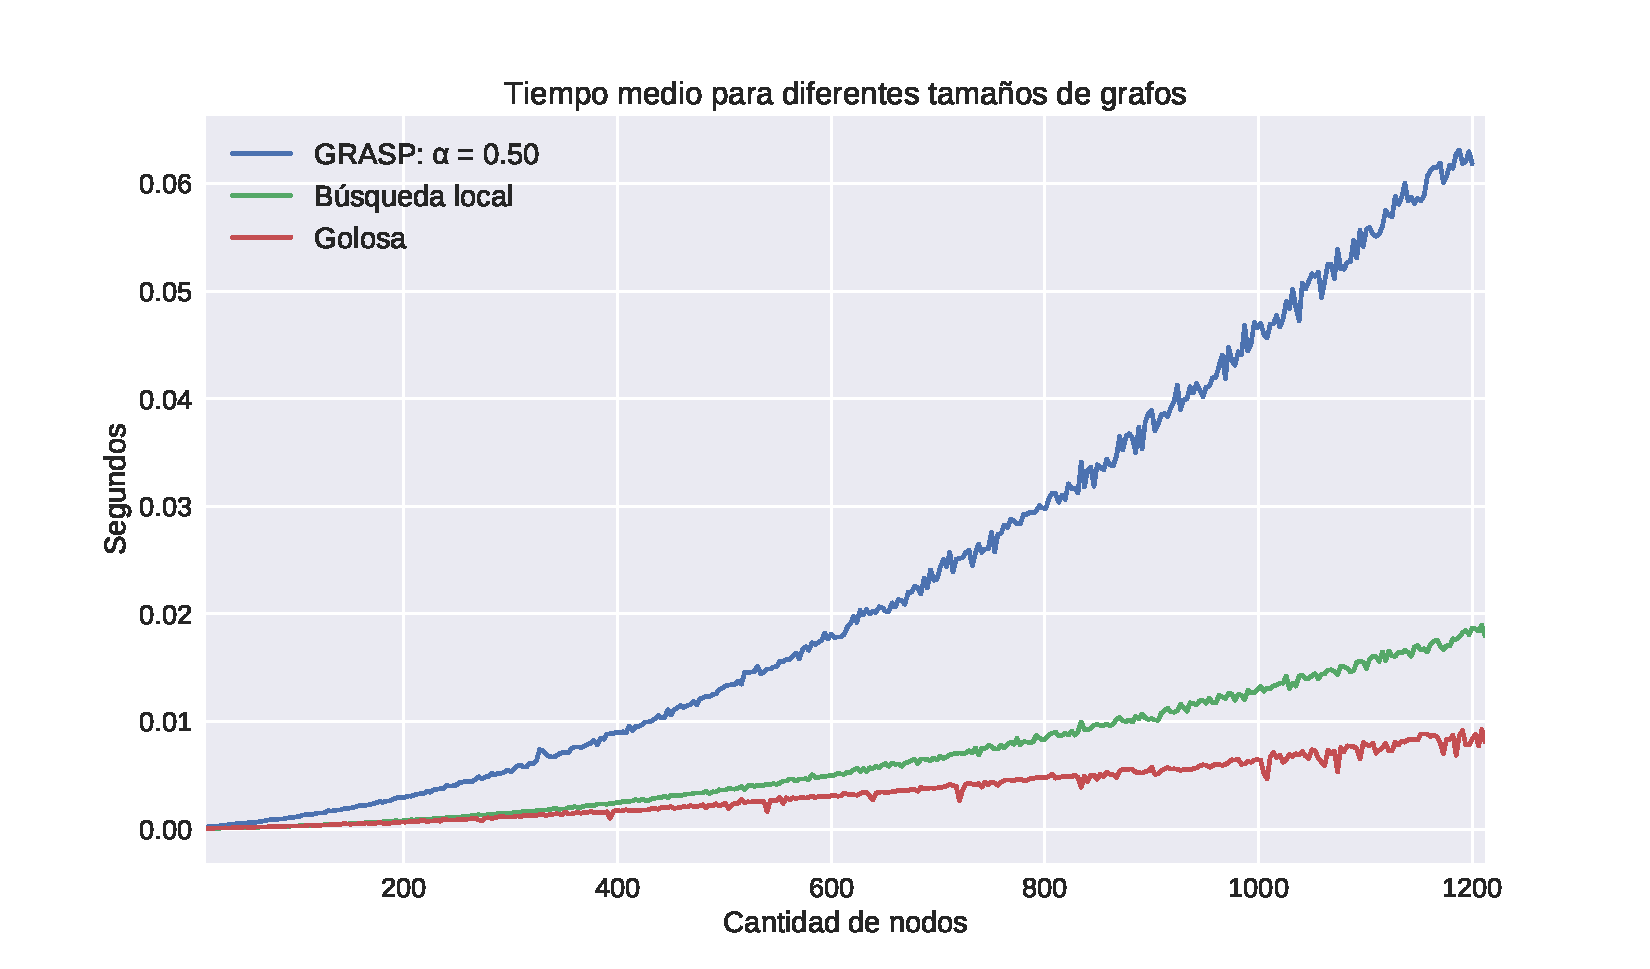
\includegraphics[width=1\textwidth]{informe/imgs/exp_malo_tiempo_grasp_local_greedy.pdf}
% }
El nivel de aleatoriedad con el que se crea la RCL del GRASP depende de nuestro parámetro $\alpha$. $\alpha = 0$ representa una elección puramente greedy, mientras que $\alpha = 1$ hace una elección puramente aleatoria. Dado que los nuestro son grafos bastantes particulares, al introducir un poco de aleatoriedad con el alpha, ya logramos obtener las mejores fronteras posibles. Puede verse que como adelantamos, cuando alpha es 0 se produce una eleccion puramente greedy, por lo que siempre es peor. \\

Es importante aclarar que esto es así por el tipo particular de grafos que estamos tratando, en el caso general esto puede no ser cierto. Intuitivamente los mejores resultados se obtienen en el equilibrio, con $\alpha = $0.5, por lo que en los siguientes casos utilizaremos este valor. \\

{\centering
    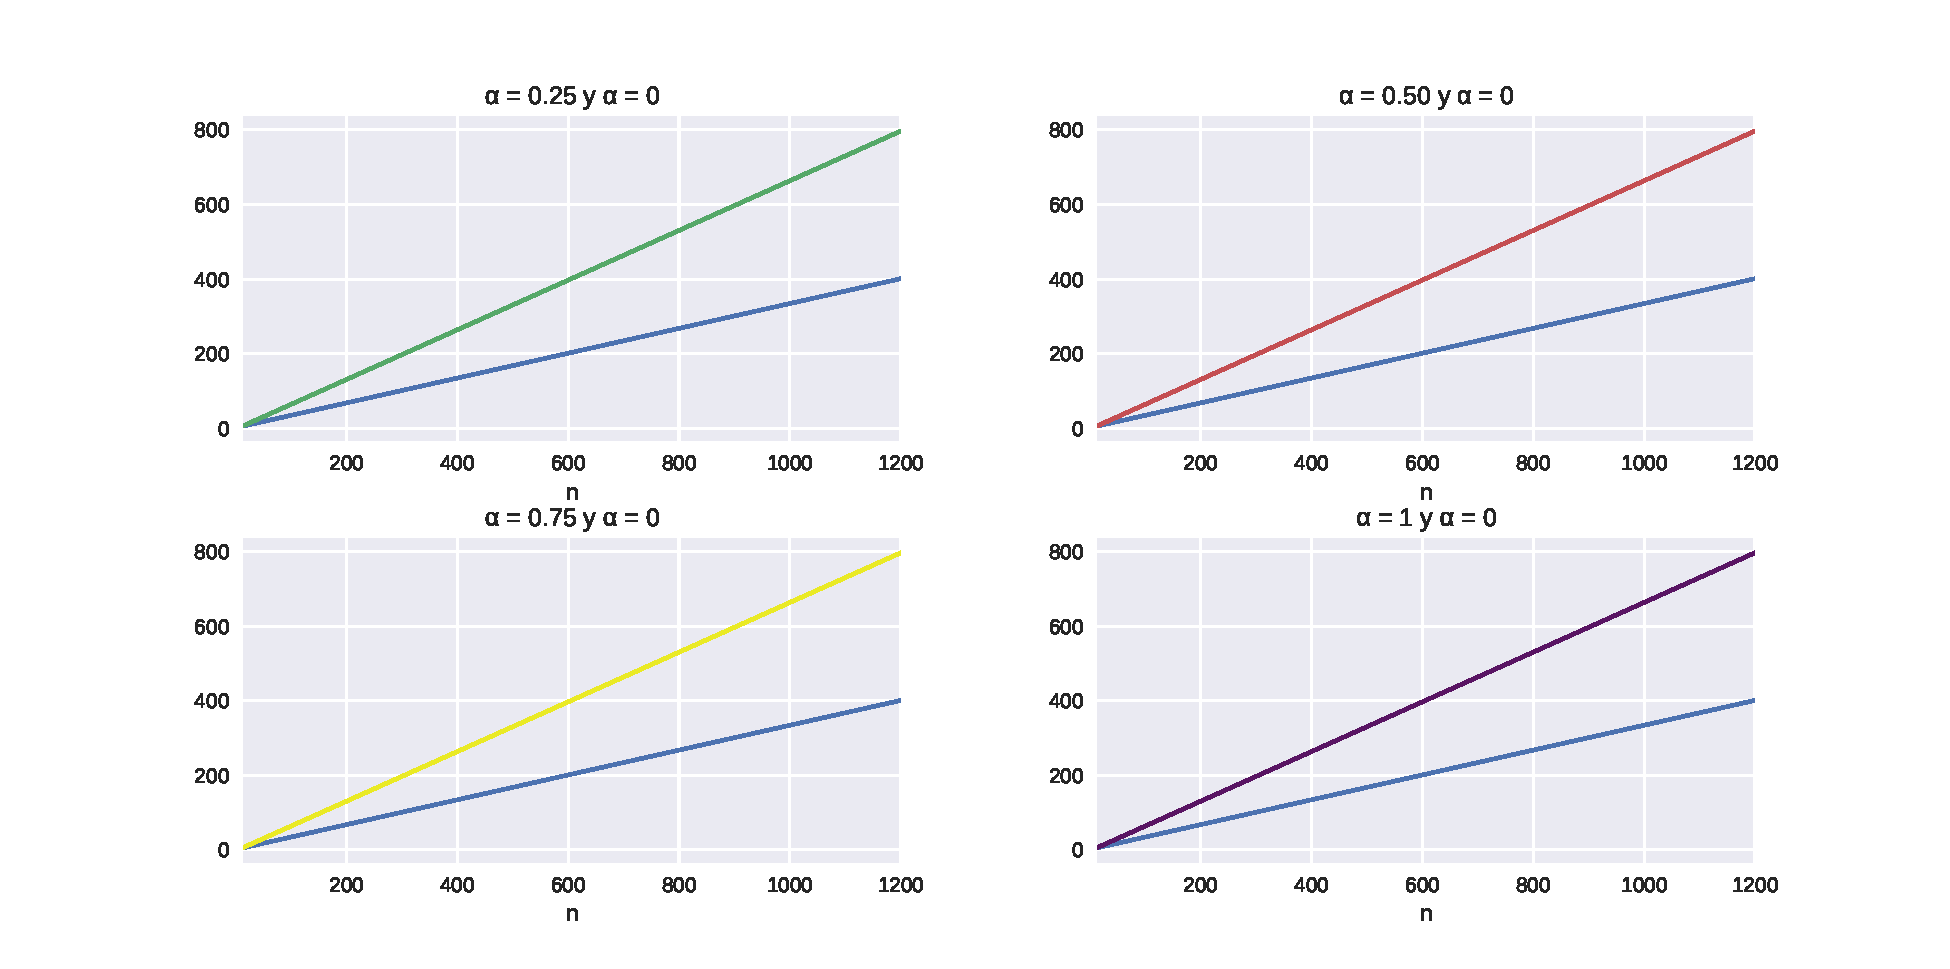
\includegraphics[width=1\textwidth]{informe/imgs/exp_malo_frontera_grasp_alphas.pdf}
}

% Esto era fruta completamente, tenia que ver con que se hacian muy pocas iteraciones de grasp y local
% {\centering
%     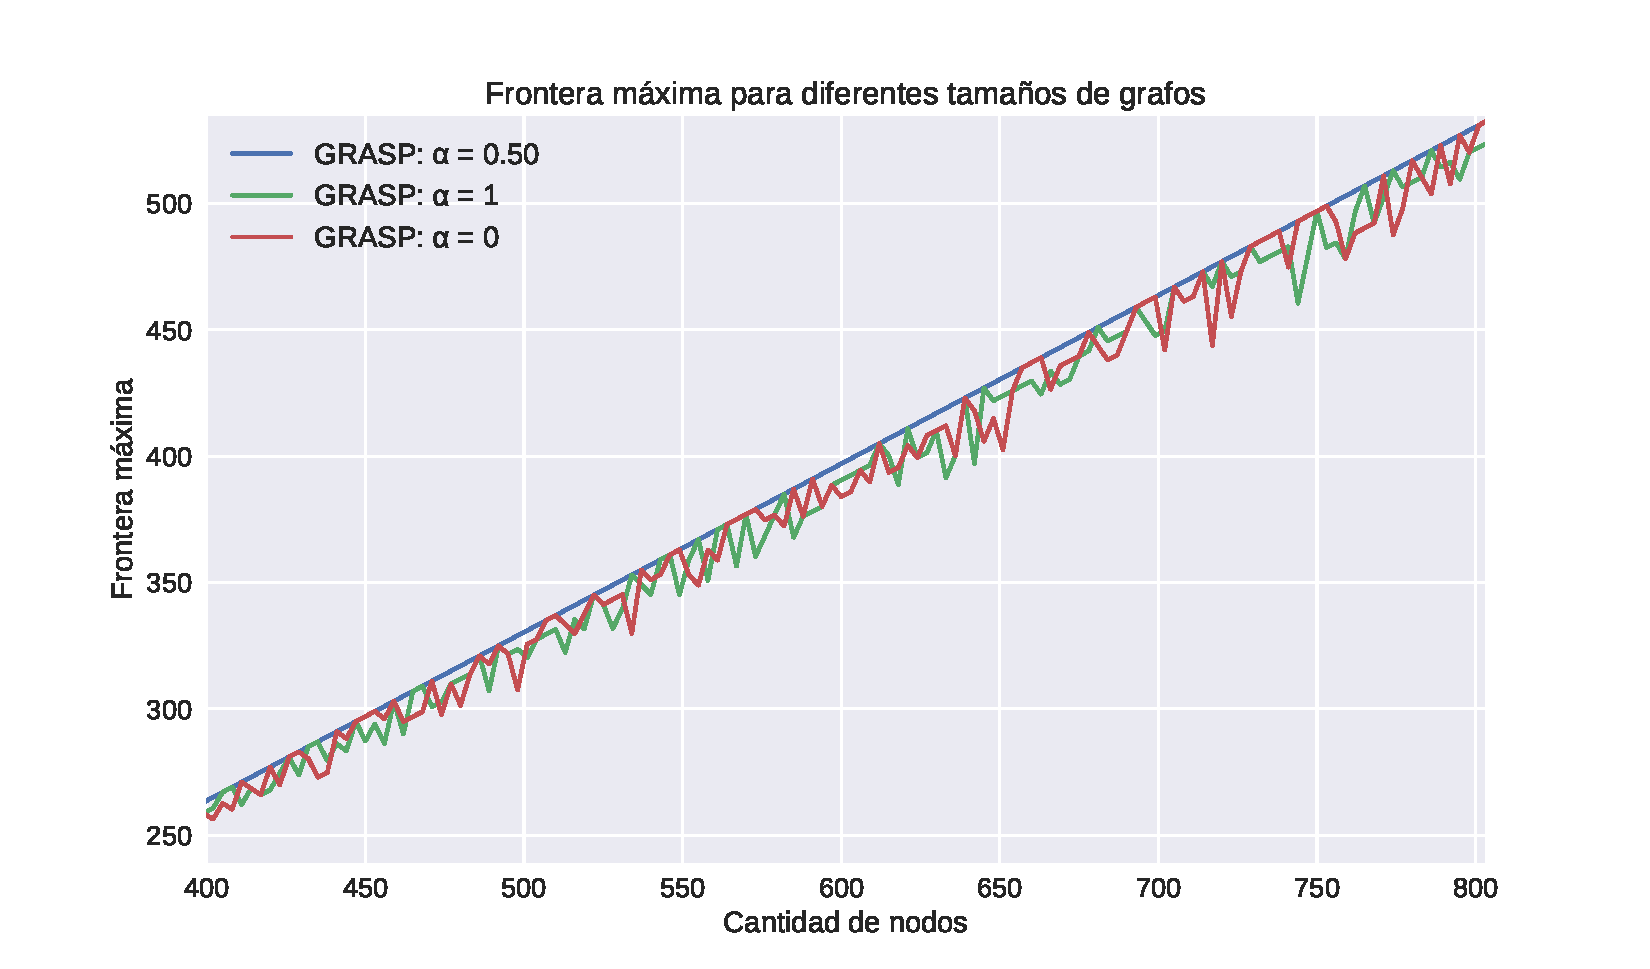
\includegraphics[width=0.90\textwidth]{informe/imgs/exp_malo_frontera_grasp_zoom.pdf}
%     % \captionof{figure}{$\uparrow$ Zoom del gráfico anterior}
% }

Otro parámetro importante es la cantidad de iteraciones a realizar, tanto en GRASP como en la búsqueda local interna. Para búsqueda local utilizamos $repsLocal = 2000$, al igual que en el apartado anterior. Con $repsGrasp$ fuimos variándolo y no encontramos ninguna diferencia apreciable, creemos que es por el tipo de grafo. Para estos experimentos tomamos $repsGrasp = 50$. \\

Nos interesa averiguar entonces qué tan lejos estamos del óptimo para nuestros ``grafos malos''. Estamos interesados en saber si la estretagia para escapar de los extremos locales funciona. Veamos lo que nos muestran los datos, recordando que anteriormente pudimos calcular cuál es la solución óptima para este tipo de grafos. \\

{\centering
    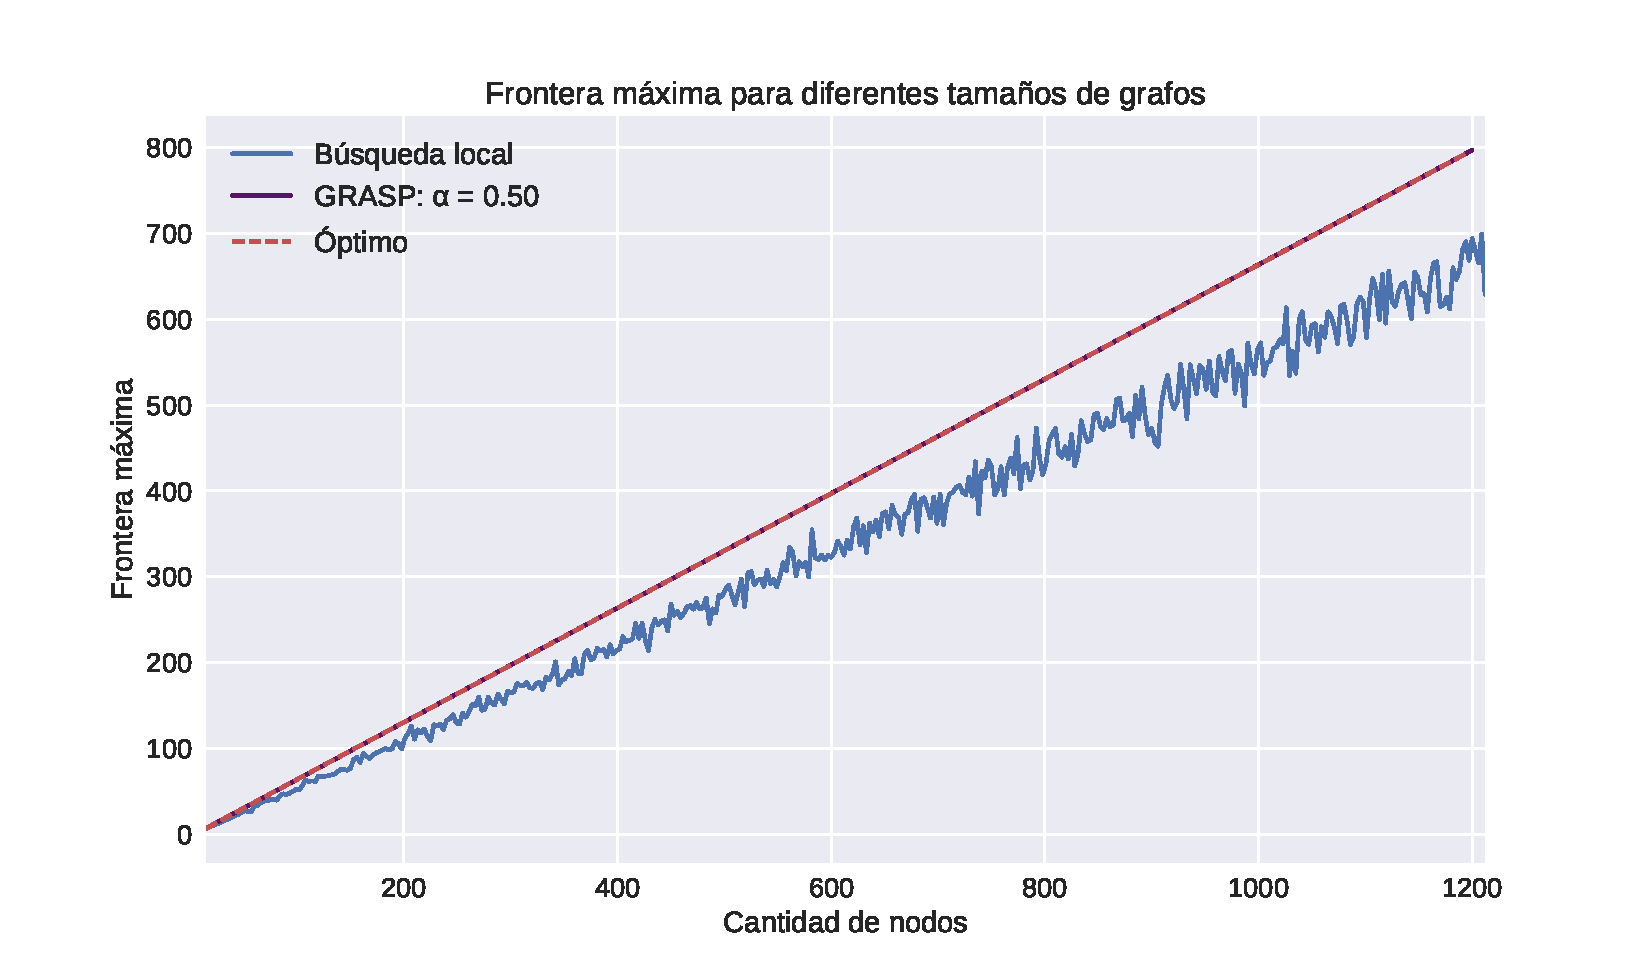
\includegraphics[width=1\textwidth]{informe/imgs/exp_malo_frontera_grasp_local_optimo.pdf}
}

La solución promedio de GRASP es \textbf{exactamente} la solución óptima! \\

Logramos resolver el problema de forma óptima para el caso en los que las demas técnicas fallaban. Es esperable que GRASP también sea bastante bueno para grafos en general. Veremos qué tan cierta es esta intuición en la siguiente sección. \\

Antes de concluir con este apartado, es interesante considerar cuál es el costo temporal de utilizar GRASP dependiendo el valor de $\alpha$. Aquí unas comparaciones:

{\centering
    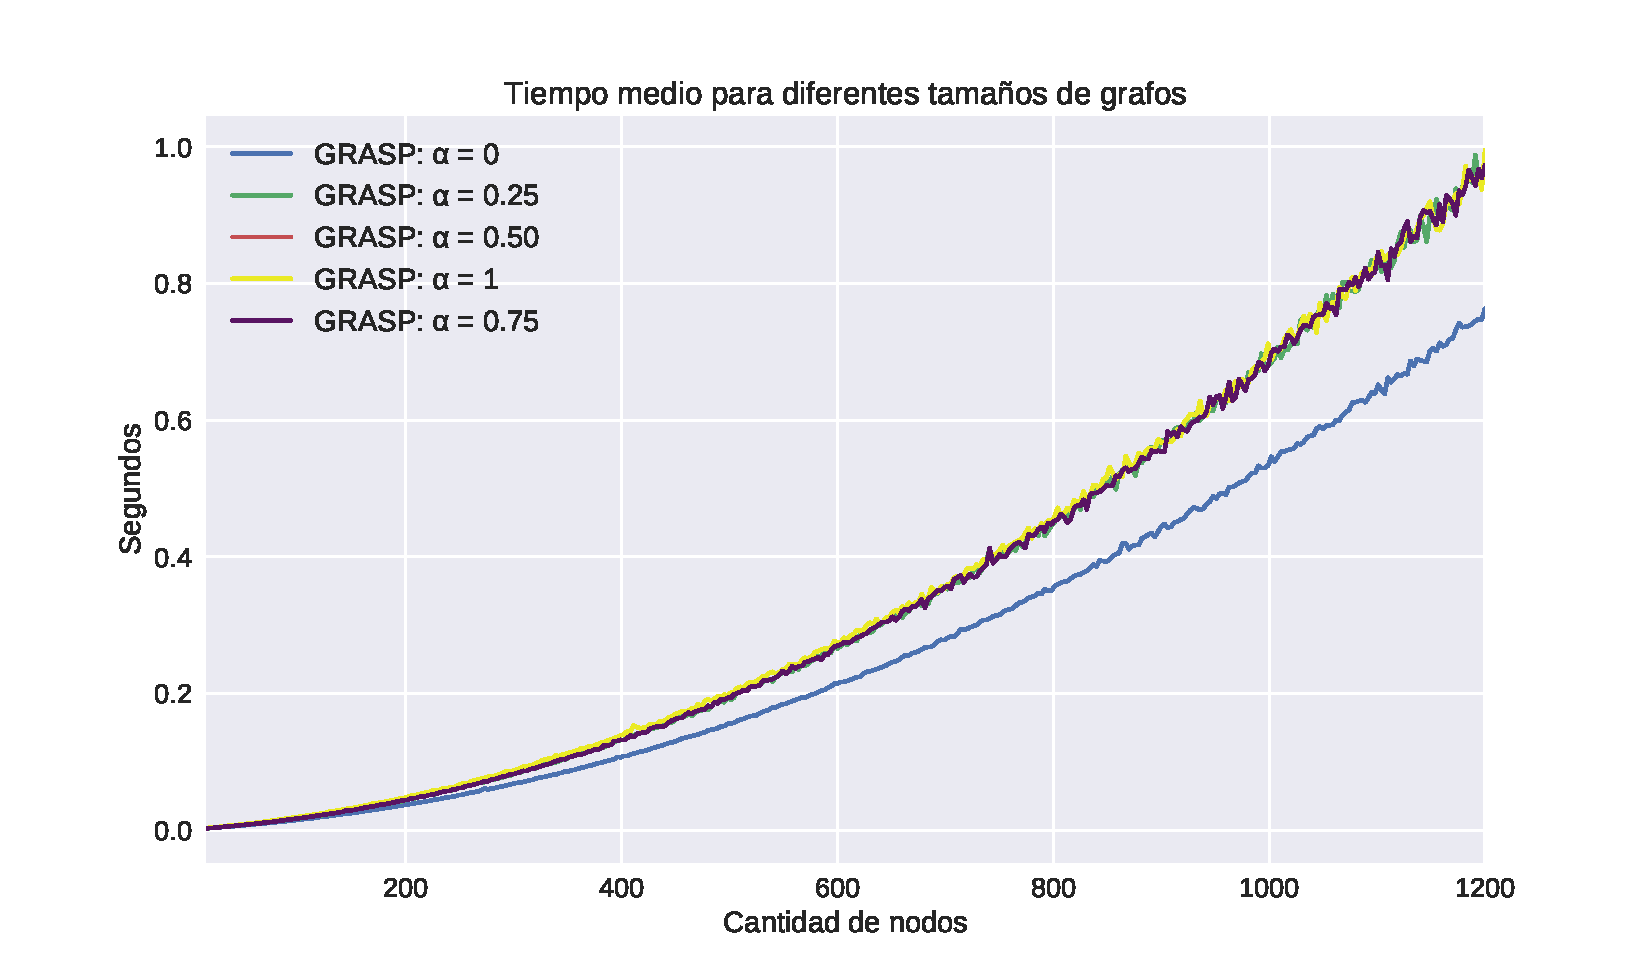
\includegraphics[width=1\textwidth]{informe/imgs/exp_malo_tiempo_grasp.pdf}
}
